
\section{球面和球面系统}
可见光是一种波长在380-760$nm$ 波段的电磁波
        \begin{figure}[H]
            \centering
            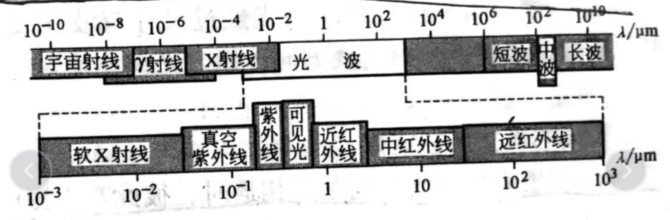
\includegraphics[width=8cm]{img/0.1.png}
            \end{figure}
\begin{quote}
{\qquad\parindent2\ccwd\kaishu\zihao{5}
虚实像物点,物像空间。
}
\end{quote}
\subsection{概念和符号系统}
\subsubsection{完善成像条件}
\begin{enumerate}[nosep]% nosep表示没有垂直间隔
    \item 同心光束成同心光束
    \item 球面波成球面波
    \item 物点像点之间等光程
\end{enumerate}
\subsubsection{一些成像中的概念}
\begin{description}[leftmargin=1.7cm,style=nextline,nosep]% nosep没有垂直间隔
    \item[同心光束] 从同一点发出的或\textbf{汇聚到同一点}的光线束。
    \item[光具组] 若干反射折射面组成的光学系统
    \item[虚实像物点] 同一点发出(实际光线汇聚)的为\textbf{实物}(像)点,汇聚(延长线汇聚)到同一点的为\textbf{虚物}(体)点。
    \item[像物方空间] 实际上,一束光经过一个光学系统,整个空间都是物方空间和像方空间,就是有虚实之分。只不过我们习惯上将像(物)实空间叫做像(物)空间。
    
    同时,符号中不带$'$ 的为物方,带的为像方。如$l,l',n,n',u,u'$。
\end{description}
\subsubsection{一些规定的概念}
\begin{description}[leftmargin=1.7cm,style=nextline,nosep]% nosep没有垂直间隔
    \item[子午平面] 包含光轴的平面
    \item[截距] 物方或像方光线与光轴交点到顶点的距离。
    \item[倾斜角] 物方或像方光线与光轴的夹角。
\end{description}
\subsubsection{约定的符号}
为了表示各种线段量和角度量的属性,我们约定俗成地规定了一些符号。
\begin{description}[leftmargin=1.7cm,style=nextline,nosep]% nosep没有垂直间隔
    \item[传播方向] 物方到像方,并且定义此方向单位向量$\vec{n}$
    \item[沿轴线段] 从折射球面顶点出发到终点(名称左到右),向量为$\vec{r}$,定义其长度为$\vec{r}\cdot \vec{n}$
    \item[垂轴线段] 光轴上正,下负。如果$\vec{n}=(x_0,y_0)$,定义$\vec{n_v}=(-y_0,x_0)$,从折射球面顶点出发到终点(名称左到右),向量为$\vec{r}$,定义其长度为$\vec{r}\cdot \vec{n_v}$
    \item[间隔$d$] 见上。对于一般角度,类比上个方法。
    \item[角度] 从\textbf{光轴到光线到法线}(\textbf{轴线法}),锐角转向,顺正逆负。
    \item[球面半径] 以球面和主光轴的交点为准到球心做向量$\vec{r}$,$r=\vec{r}\cdot \vec{n}$。如右图,其为
    $$
    L_{OC}
    $$
\end{description}

\subsection{基本公式和定理}
$$
n=\frac{c}{v}
$$
\begin{theorem}[费马原理]
光是沿着光程取极值的路径传播的(极大值、极小值或常数)。
\end{theorem}
\begin{theorem}[马吕斯定律]
    光线束在\textbf{各向同性的均匀介质中}传播时,始终保持着与波面的正交性,并且入射波面与出射波面对应点之间的光程均为定值。
\end{theorem}
几何光学有三个基本定律,分别是\textbf{光的直线传播,光的独立传播,光的折反射定律}。
\subsubsection{光的直线传播} 在各向同性的介质中,不遇到波长量级的障碍物时(衍射),光沿直线传播。
\subsubsection{光的独立传播} 不同光源发出的光,在空间某点相遇时,彼此互不影响。(同一单色点光源,干涉)
\subsubsection{光的折反射定律}
\begin{itemize}
\item 全反射是从光密到光疏,入射角大于临界角。
\item 对于反射
$$ n'=-n
$$
\item 对于折射
$$
n\sin I=n'\sin I'
$$
\begin{quote}
{\qquad\parindent2\ccwd\kaishu\zihao{5}
注意$I,I'$ 是入射和出射和法线所成角。
}
\end{quote}
\end{itemize}
\subsection{基本公式推导(单球面折射)}
我们需要根据入射光线给出的条件$r,n,n',L,U$,求出$L',U'$
\begin{figure}[H]
    \centering
    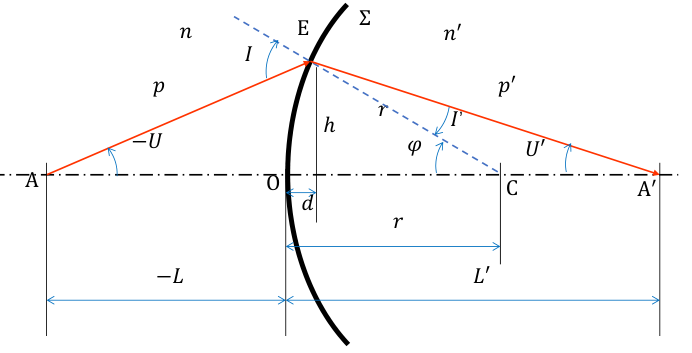
\includegraphics[width=8cm]{img/1.1.png}
\end{figure}
根据折射定律得
\begin{equation}
    n \sin I =n' \sin I '\tag{1.2.1.a}
\end{equation}
在$\Delta EAC$ 中运用正弦定理,得到
\begin{equation}
    \frac{\sin I }{r-L}=\frac{\sin -U}{r}\tag{1.2.2.a}
\end{equation}
显然又因为内外角定理,可得
\begin{equation}
    \varphi=U+I=U'+I' \tag{1.2.3.a}
\end{equation}
在$\Delta ACE$ 中再使用正弦定理,可得
\begin{equation}
    L'=r+\frac{r}{\sin U'} \sin I' \tag{1.2.4.a}
\end{equation}
显然固定$L,r,n,n'$,动$U$,显然$L'$会发生改变,即不是同心光束,
不能\textbf{完善成像}。
\subsubsection{近轴光路近似}

\begin{description}[leftmargin=1cm,style=nextline,nosep]% nosep没有垂直间隔
    \item[近轴(傍轴)光线] 与光轴很靠近的光线,即-U很小,此时\textbf{用小写
            (如-u等)}表示近轴光线的参数。
\end{description}
此时可利用小角近似,$i=\sin i= \tan i$,所以(1.2.1.a-1.2.4.a)可以写成
\begin{align}
    n i =n' i '\tag{1.2.1.b}                 \\
    \frac{i }{r-l}=\frac{-u}{r}\tag{1.2.2.b} \\
    \varphi=u+i=u'+i' \tag{1.2.3.b}          \\
    l'=r+\frac{r}{ u'}  i' \tag{1.2.4.b}
\end{align}
化简(1.2.4.b)
\begin{equation}
    \begin{aligned}
        l'=r+r \frac{i'}{u'} & =r+r \frac{i'}{u+i-i'}                       \\
                             & =r+r \frac{\frac{n}{n'}i}{u+i-\frac{n}{n'}i} \\
                             & =r+r \frac{n}{\frac{n'u}{i}+n'-n}
    \end{aligned}
    \tag{1.2.5}
\end{equation}
先算$i$
\begin{equation}
    i= \frac{u(l-r)}{r}\tag{1.2.6}
\end{equation}
(1.2.6) 代入(1.2.5)
\begin{equation}
    l'=r+r \frac{n}{\frac{n'r}{l-r}+n'-n}\tag{1.2.7}
\end{equation}
显然$l'$与$u$无关,其\textbf{完善成像}。此时的像物点又叫做\textbf{共轭点}。
近轴光所成像称为\textbf{高斯像},
仅考虑近轴光的光学叫\textbf{高斯光学}。
\subsubsection{近轴光路其他公式}
\begin{figure}[H]
    \centering
    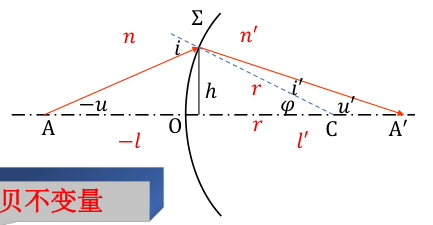
\includegraphics[width=7cm]{img/1.2.png}
\end{figure}
我们新引入了一个$h$,先来引入几个关于它的式子
\begin{align}
    h       & =lu=l'u' \tag{1.2.8}                               \\
    \varphi & \thickapprox \tan \varphi= \frac{h}{r} \tag{1.2.9}
\end{align}
Then Let,s start our solve
\begin{description}[leftmargin=0.7cm,style=nextline,nosep]% nosep没有垂直间隔
    \item[折射球面的物像位置关系]
        由(1.2.8)得,\begin{equation}
            u=\frac{h}{l} \quad u'=\frac{h}{l'} \tag{1.2.10}
        \end{equation}
        化简(1.2.1.b)得{1.2.11.a},其移项化简可得后一项
        \begin{align}
            n(\varphi-u)=n'(\varphi-u') \tag{1.2.11.a} \\
            n u-n' u'=(n-n')\varphi =(n-n')\frac{h}{r} \tag{1.2.11.b}
        \end{align}
        将(1.2.10)代入(1.2.11.b),可得
        \begin{equation}
            \frac{h}{l}n-\frac{h}{l'}n'=(n-n')\frac{h}{r}\tag{1.2.12.bef}\footnote{bef表示该公式的前置证明步骤公式}。
        \end{equation}
        \begin{equation}
            \frac{n}{l}-\frac{n'}{l'}=\frac{n-n'}{r}\tag{1.2.12}
        \end{equation}
        此式即为\textbf{折射球面的物像位置关系},同时,此式也可由式(1.2.7)直接化简而来.下面简要说明
        \begin{equation}
            \begin{aligned}
                l'&=r+r(\frac{n}{\frac{n'r}{l-r}+n'-n})\\
                &=r(1+\frac{nl-nr}{n'r+(n'-n)(l-r)})\\
                &=r(1+\frac{nl-nr}{n'l-nl+nr})\\
                &=r(\frac{n'l}{n'l-nl+nr})
               \end{aligned} \tag{1.2.12.af1}
        \end{equation}
        继续化简
        \begin{align}
         rn'l=(n'&-n)ll'+rnl' \tag{1.2.12.af 2} \\
         r(n'l-nl')&=(n'-n)ll' \tag{1.2.12.af 3}\\
         \frac{n'}{l'}-\frac{n}{l}&=\frac{n'-n}{r} \tag{1.2.12.af 4}   
        \end{align}
        \item[阿贝不变量]
        化简(1.2.11.a)
        \begin{align}
            n(\frac{h}{r}-\frac{h}{l})=n'(\frac{h}{r}-\frac{h}{l'}) \tag{1.2.13.bef} \\
            n(\frac{1}{r}-\frac{1}{l})=n'(\frac{1}{r}-\frac{1}{l'}) =Q \tag{1.2.13}
        \end{align}
        式(1.2.13)即为\textbf{阿贝不变量}公式。
    \item[光焦度]
        表示折射面偏折光线的能力
        \begin{equation}
            \Phi=\frac{n'-n}{r}\tag{1.2.14}
        \end{equation}
    \item[焦距]
        \begin{align}
            \frac{1}{f}=\frac{1}{l_{l' \to \infty}} & =\frac{n-n'}{nr} \tag{1.2.15.a}   \\
            \frac{1}{f'}=\frac{1}{l_{l \to \infty}} & =-\frac{n-n'}{n'r} \tag{1.2.15.b}
        \end{align}
        用光焦度表示的焦距
        \begin{equation}
            \frac{1}{f}= -\frac{1}{n} \Phi\hspace{0.5cm}  \frac{1}{f'}=\frac{1}{n'}\Phi\tag{1.2.16}
        \end{equation}
        化简上述公式可得
        \begin{equation}
            \frac{f'}{f}=-\frac{n'}{n}\tag{1.2.17}
        \end{equation}
        $\displaystyle \frac{1}{(1.2.15.a)}+\frac{1}{(1.2.15.b)}$可得
        \begin{equation}
            f+f'=\frac{1}{r}\tag{1.2.18}
        \end{equation}
        如果对于空气中(理想光学系统),$n=1$就有
        \begin{align}
                f+f'&=\frac{1}{r}=0\tag{1.2.18.a}\\
                \Phi&=-\frac{1}{f}=\frac{1}{f'}\tag{1.2.16.a}
        \end{align}

    \item[屈光度]
        光焦度的单位称为\textbf{屈光度},以字母D表示(对应焦距单位:米)
        \begin{enumerate}[nosep]% nosep表示没有垂直间隔
            \item  200度近视镜光焦度-2.00D(凹透镜)\textcolor{red}{\textbf{负透镜}}
            \item 300度老花镜光焦度3.00D(凸透镜)\textcolor{red}{\textbf{正透镜}}
        \end{enumerate}
    \item[高斯公式]
        将(1.2.15.a),(1.2.15.b)代入式(1.2.12)得
        \begin{equation}
            \frac{n-n'}{r}=\frac{(n-n')f}{rl}+\frac{(n-n')f'}{rl'}  \tag{1.2.19.bre1}
        \end{equation}
        显然可得
        \begin{equation}
            \frac{f}{l}+\frac{f'}{l'}=1 \tag{1.2.19}
        \end{equation}
        式(1.2.19)即为\textbf{高斯公式}。

    \item[牛顿公式]
    设A为物垂点,$A'$为像点垂点,$\displaystyle x=l_{FA},x'=l_{F'A'}$(见下图1.1),有
  \begin{align}
 l&=x+f \tag{1.ad.1.a} \\
 l'&=x'+f' \tag{1.ad.1.b}
  \end{align}
将(1.ad.1.a),(1.ad.1.b)代入式(1.2.19)得
\begin{align}
    \frac{f}{x+f}&+\frac{f'}{x'+f'}=1 \tag{1.ad.2.bef.1} \\
    x'f+2ff'+xf'&=xx'+ff'+x'f+xf' \tag{1.ad.2.bef.2}\\
    ff'&=xx' \tag{1.ad.2}
\end{align}
    % \item[]
\end{description}
\subsubsection{三种放大率和拉氏不变量}
        \begin{figure}[H]
            \centering
            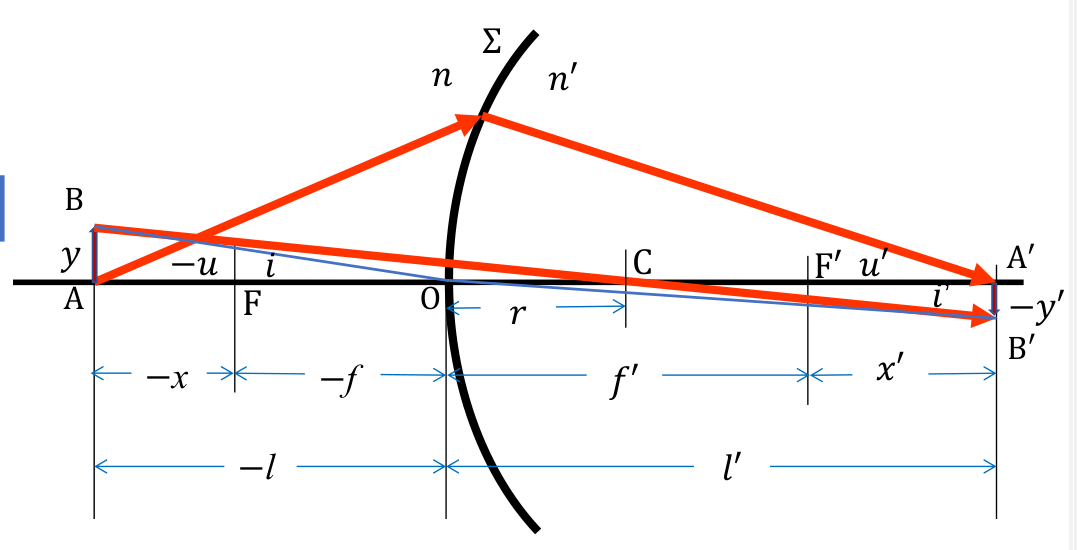
\includegraphics[width=8cm]{img/1.3.png}
            \caption[图1.1]{光路示意图}
            \end{figure}
% 上图中存在错误,我们将图中的$-l$ 记作$l$,$-y'$ 记作$y'$ 注意其均\textbf{带有正负}.
\begin{description}[leftmargin=0.7cm,style=nextline,nosep]% nosep没有垂直间隔
    \item[横向放大率] 
     \begin{equation}
     \beta=\frac{y'}{y}=\frac{l'i'}{li}\tag{1.2.20}
     \end{equation}
     又因为有
\begin{align}
    ni=ni' \quad lu=l'u' \tag{1.2.21.bre 1}\\
        nlui=n'l'u'i'  \tag{1.2.21.bre 2}
\end{align}
所以可得
\begin{equation}
\beta=\frac{nu}{n'u'}=\frac{nl'}{n'l} \tag{1.2.21}
\end{equation}
继续化简
\begin{equation}
\begin{aligned}
    \beta=-\frac{fl'}{f'l}&=-\frac{f(x'+f')}{f'(x+f)}
    \\
    &=-\frac{fx'+xx'}{f'(x+f)}=-\frac{x'}{f'}\\
    &=-\frac{f(x'+f')}{f'x+xx'}=-\frac{f}{x}
\end{aligned}
\tag{1.ad.3}
\end{equation}
\begin{quote}
{\parindent2\ccwd\kaishu\zihao{5}
$\beta>0$正立虚实相反像,$\beta<0$倒立虚实相同像。>1放大,<1缩小。
}
\end{quote}
    \item[横向(垂轴)放大率] 
    \begin{equation}
    \alpha=\frac{\mathrm{d}{ l'}}{\mathrm{d}{l}} \tag{1.2.22.a}
    \end{equation}
    (1.2.12)两端分别对$u$进行求导,r对u是常数,所以有
    \begin{align}
      \frac{n'}{l'^2}\frac{\mathrm{d}{l'}}{\mathrm{d}{u}}-\frac{n}{l^2}\frac{\mathrm{d}{l}}{\mathrm{d}{u}}=0 \tag{1.2.22.bef 1}\\ 
      \frac{n'}{l'^2}\frac{\mathrm{d}{l'}}{1}=\frac{n}{l^2}\frac{\mathrm{d}{l}}{1}\tag{1.2.22.bef 1}
    \end{align}
    所以求得
    \begin{equation}
    \alpha=\frac{\mathrm{d}{l'}}{\mathrm{d}{l}}=\frac{nl'^2}{n'l^2}=\frac{\beta^2}{\frac{n}{n'}}=\frac{n'}{n}\beta^2 \tag{1.2.22}
    \end{equation}

    % 或者有一种更为简单的推导方法,使用(1.ad.2),可得
    \item[角放大率]
    \begin{equation}
    \gamma=\frac{u'}{u}=\frac{l}{l'}=\frac{1}{\beta}\frac{n}{n'} \tag{1.2.23}
    \end{equation} 
    或者说
    \begin{equation}
    \beta=\frac{nu}{n'u'}=\frac{n}{n'} \frac{1}{\gamma} \tag{1.add.4}
    \end{equation}
\end{description}
显然以上三种放大率$\alpha \hspace{0.2cm}  \beta\hspace{0.2cm}   \gamma$之间存在关系,
\begin{equation}
\alpha\gamma=\beta\tag{1.2.24}
\end{equation}
\begin{description}[leftmargin=0.7cm,style=nextline,nosep]% nosep没有垂直间隔
    \item[拉式不变量] 同时根据$\beta$我们定义一个叫做拉式不变量的概念
    \begin{align}
    \frac{y'}{y}=\beta=\frac{nu}{n'u'}    \tag{1.2.25.bef 1}\\
      nuy=n'u'y'=j  \tag{1.2.25}
    \end{align}
    j为拉氏不变量,它是表征光学系统性能的重要参数
\end{description}

\subsection{反射球面}\
其实就是将$n+n'=0$代入上述所有基本公式进行化简,下面给出部分常用公式
\begin{align}
\Phi&=\frac{-2n}{r}=\frac{2n'}{r} \tag{1.2.26} \\
f&=f'=\frac{r}{2} \tag{1.2.27} \\
&\frac{1}{l}+\frac{1}{l'}=\frac{2}{r} \tag{1.2.28}
\end{align}
% \subsection{共轴球面系统}
% \subsection{透镜}
\section{薄透镜理想光学系统}
\subsection{共轴球面系统}
\begin{figure}[H]
    \centering
    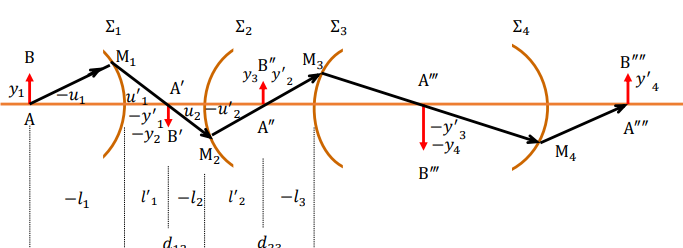
\includegraphics[width=8cm]{img/1.4.png}
    \end{figure}
    \subsubsection{过渡公式}
第$i$面的物方空间就是第$i+1$面的像方空间。所以
\begin{align}
    n_{i+1}&=n'_{i} \tag{2.add.1.a}\\
     u_{i+1}&=u'_{i} \tag{2.add.1.b}\\
     y_{i+1}&=y'_{i} \tag{2.add.1.c} 
\end{align}
同时有
\begin{align}
d_i=d_{i(i+1)}&=l_{i}'-l_{i+1} \tag{2.add.2.pre} \\
l_{i+1}&=l_{i}'-d_i \tag{2.add.2}
\end{align}
(2.add.2)乘(2.add.1.b)可得($h_i=l_iu_i$)
\begin{equation}
h_{i+1}=h_i-d_i u_{i}'\tag{2.add.3}
\end{equation}
对每个面应用拉式不变量和过度公式(2.add.1)可得
\begin{align}
    n_iu_iy_i=J \tag{2.add.4}
\end{align}
       
\subsubsection{放大率}
\begin{align}
    \alpha_n=\frac{\mathrm{d}{l'_n}}{\mathrm{d}{l_1}}=\prod_{i=1}^n \alpha_i \tag{2.1.1.a}\\
    \beta_n=\frac{y_n'}{y_1}=\prod_{i=1}^n \beta_i \tag{2.1.1.b}\\
    \gamma_n=\frac{u_n'}{u_1}=\prod_{i=1}^n \gamma_i \tag{2.1.1.c}
\end{align}
其关系顺延之前。
\subsection{薄透镜}
\begin{description}[leftmargin=0.7cm,style=nextline,nosep]% nosep没有垂直间隔
    \item[薄透镜] 透镜厚度d 远小于物距、像距、焦距、曲率半径等 
       \begin{figure}[H]
                \centering
                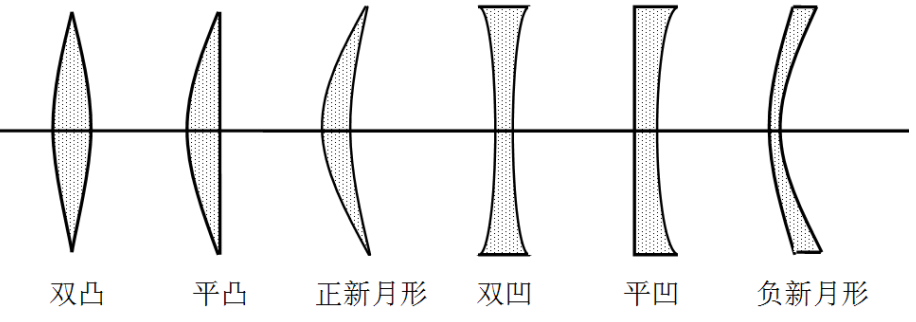
\includegraphics[width=8cm]{img/1.5.png}
                \end{figure}
\end{description}
\subsubsection{成像}        \begin{figure}[H]
            \centering
            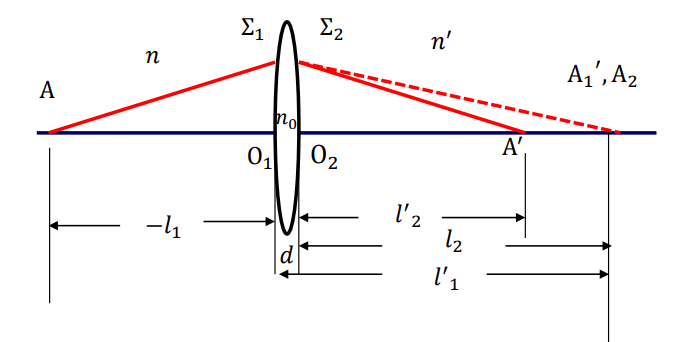
\includegraphics[width=8cm]{img/1.7.png}
            \end{figure}
\begin{align}
    \frac{n_0}{l_1'}-\frac{n}{l_1}=\frac{n_0-n}{r_1} \tag{2.2.1.a}\\
    \frac{n'}{l_2'}-\frac{n_0}{l_2}=\frac{n'-n_0}{r_2} \tag{2.2.1.b}
\end{align}
并且
\begin{equation}
l_2=l_1'+d \thickapprox  l_1' \tag{2.2.2}
\end{equation}
(2.2.1.a)+(2.2.1.b)
\begin{align}
    \frac{n'}{l_2'}-\frac{n}{l_1}=\frac{n_0-n}{r_1}+\frac{n'-n_0}{r_2}\tag{2.2.3.a}\\
    \frac{n'}{l'}-\frac{n}{l_1}=\frac{n_0-n}{r_1}+\frac{n'-n_0}{r_2}\tag{2.2.3.b}
\end{align}
(2.2.3.b) 就是\textbf{薄透镜傍轴成像的物像距公式}。化简一下
\begin{equation}
    n(\frac{1}{r_1}-\frac{1}{l})-n'(\frac{1}{r_2}-\frac{1}{l'})=n_0(\frac{1}{r_1}-\frac{1}{r_2}) \tag{2.2.4}
\end{equation}
设(2.2.3.b)等式右边为$\Phi$,可得
\begin{align}
\text{物方焦距}f=\lim_{l' \to \infty}\frac{-n}{\Phi} \tag{2.2.5.a}\\
\text{像方焦距}f'=\lim_{l \to \infty}\frac{n'}{\Phi} \tag{2.2.5.b}\\
f=-f'=\frac{n}{\Phi} \tag{2.2.5.c}
\end{align}
$f'>0$汇聚$<0$发散。联立以上各方程组,可得其牛顿公式和高斯公式基本不变
\begin{align}
    \text{高斯公式}\frac{f'}{l'}+\frac{f}{l}=1 \tag{2.2.6.a}\\
    \text{牛顿公式}xx'=ff' \tag{2.2.6.b}
\end{align}

并且如果在空气中$n=n'=1$,可得
\begin{align}
f'=-f=\frac{1}{\Phi} \tag{2.2.7.a}\\
\Phi=(n_0-1)(\frac{1}{r_1}-\frac{1}{r_2}) \tag{2.2.7.b}
\end{align}
$\displaystyle \Phi>0,\frac{1}{r_1}-\frac{1}{r_2}>0$ 凸透镜,反之凹透镜。(其实只考虑两种最极端的情况就行)
对于放大率来说,
\begin{align}
 \beta_1=\frac{n_1l_1'}{n_1'l_1} \tag{2.2.8.a}\\
 \beta_2=\frac{n_2l_2'}{n_2'l_2} \tag{2.2.8.b}\\
 \beta=\beta_1 \beta_2=\frac{n_1n_2l_1'l_2'}{n_1'n_2'l_1l_2} \tag{2.2.8.c}\\
 l_1'=l_2,l_1=l,l_2'=l'\tag{2.2.8.d}\\
 n_1=n,n_2'=n',n_1'=n_2=n_0\tag{2.2.8.e}
\end{align}
联立以上五式可得
\begin{equation}
\beta=\frac{nl'}{n'l}=-\frac{fl'}{f'l} \tag{2.2.9}
\end{equation}
注意上式中$f,f'$的顺序
$$
fn'+f'n=0
$$
下面再来看几个放大率,一样的分析方法(略去一点推导)
        \begin{figure}[H]
            \centering
            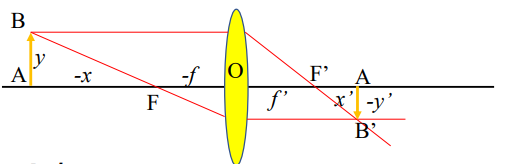
\includegraphics[width=8cm]{img/1.8.png}
            \end{figure}
            \begin{align}
                -\frac{y'}{y}=\frac{f}{x}=\frac{x'}{f'} \tag{2.2.10.a}\\
                \beta=\frac{y'}{y}=-\frac{f}{x}=-\frac{x'}{f'} \tag{2.2.10.b}
            \end{align}
            然后一如既往的
            \begin{align}
                \alpha=\frac{n'}{n}\beta^2 \tag{2.2.11.a}\\
                \gamma=\frac{n}{n'}\frac{1}{\beta}\tag{2.2.11.b}\\
                \alpha \gamma=\beta \tag{2.2.11.c}
            \end{align}
\textcolor{red}{\textbf{注意算透镜的时候,多用焦距,这样十分简单。}}
        \begin{figure}[H]
            \centering
            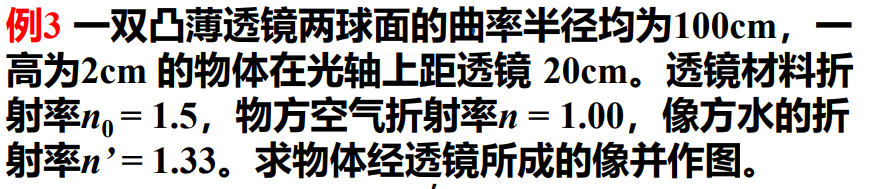
\includegraphics[width=8cm]{img/1.9.png}
            
\includegraphics[width=8cm]{img/1.10.png}

            \end{figure}
\section{理想光学系统}
单个折射球面或者是单薄透镜是对细小平面以细光束成完善像,但是实际的光学系统
需要对一定大小的场以宽光束成像,其\textbf{成像有缺陷}。所以其必须要由若干元件组成,经过反复计算,使其成像\textbf{趋于}完善。

并且对于理想光学系统,所成的像是完全相似的。这种理想光学系统理论,也被称作\textbf{高斯光学}。并且引出共轭的表示
\begin{align}
    \text{点} \to \text{共轭点} \tag{3.0.a}\\
    \text{线} \to \text{共轭线} \tag{3.0.b}\\
    \text{面} \to \text{共轭面} \tag{3.0.c}\\
    \text{同心光束} \to \text{共轭同心光束} \tag{3.0.d}
\end{align}
\subsection{共线成像理论}
由于系统的对称性,理想共轴光学系统有如下性质
\begin{description}[leftmargin=1.7cm,style=nextline,nosep]% nosep没有垂直间隔
    \item[光轴] 光轴物点的共轭点还在光轴上
    \item[子午平面] 通过光轴的平面,物点的共轭点在一子午平面上
    \item[垂轴平面] 物面垂轴,其共轭像面一定也垂轴,并且几何形状相似。
    \item[表示] 如果已知两对共轭平面的位置和$\beta$,或者一对共轭平面的位置和$\beta$,以及一对共轭点,则一切物点的像点均可确定。    
    \item[同心] 同心光束还是同心光束(理想成像) 
\end{description}
        \begin{figure}[H]
            \centering
            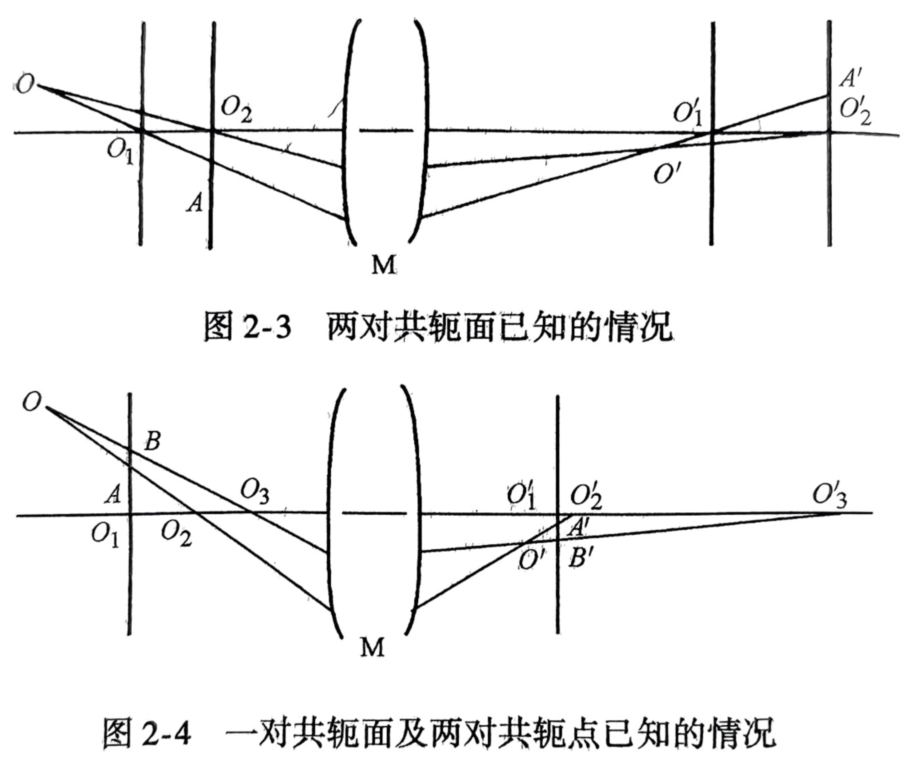
\includegraphics[width=6cm]{img/2.1.png}
            \end{figure}
\subsection{各种定义}

\subsubsection{对于无限物点}
无限远\textbf{轴上}物点发出的同心光束等效于平行于光轴的平行光束,其共轭像点为$F'$。对于轴外的话,就是下图所示
        \begin{figure}[H]
            \centering
            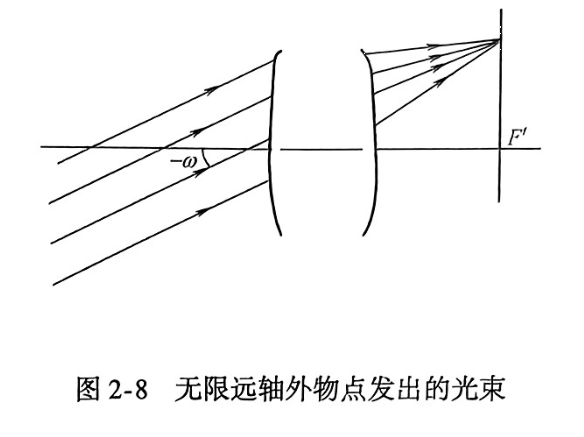
\includegraphics[width=7cm]{img/3.10.png}
            \end{figure}
\subsubsection{对于无限像点}
同上
\subsubsection{焦点和焦面}
        \begin{figure}[H]
            \centering
            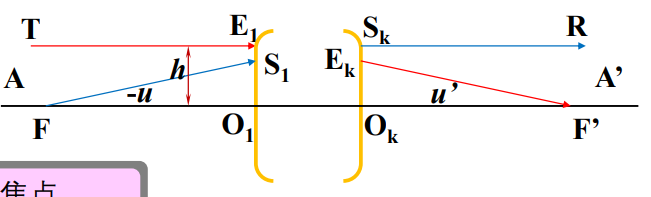
\includegraphics[width=8cm]{img/1.11.png}
            \end{figure}
            对于无穷远轴上像物点$A',A$

            \begin{align}
        A \to F' \tag{3.2.1.a} \\
        F \to A' \tag{3.2.1.b} 
    \end{align}
    物方无穷远垂轴平面的共轭平面为通过 F’的垂轴平面(后焦平面,像方焦面),像方无穷远垂轴平面的共轭平面为物方过 F 的垂轴平面(前焦平面,物方焦面)。
\begin{quote}
{\parindent2\ccwd\kaishu\zihao{5}
物方无穷远垂轴平面一轴外点,其所成平行光一定交于后焦平面一点。显然此两平面共轭。像方同理。
}
\end{quote}
\begin{align}
f=\frac{h}{\tan U} \tag{3.2.2.a}\\
f=\frac{h}{\tan U'} \tag{3.2.2.b}
\end{align}
\footnote[1]{这时候用大写的,因为有轴外物点,其不再满足前文所述\textbf{傍轴条件}}
    \subsubsection{主点$H,H'$和主平面}
    \begin{definition}[主平面]
    $\beta=1$ 的一对平面
    \end{definition}
    \begin{figure}[H]
        \centering
        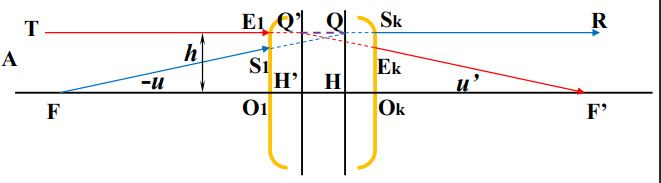
\includegraphics[width=7cm]{img/3.1.png}
        \end{figure} 
如图所示找到$Q,Q',H,H'$
\begin{align}
    Q \to Q' \tag{3.2.3.a}\\
    H \to H' \tag{3.2.3.b}\\
    QH \to QH' \quad (\beta=1) \tag{3.2.3.c}\end{align}
\begin{quote}
{\parindent2\ccwd\kaishu\zihao{5}
主点H,带不带'取决于其经过是像方焦点还是物方焦点。显然对于正透镜,左边是$H'$,对于负透镜,$f'< 0$,左边是$H$

}
\end{quote}
% \subsubsection{焦距}
% \begin{align}
% f'=\overline{H'F'}=\frac{h}{u'} \tag{2.3.3.a}\\
% f=\overline{HF}=\frac{h}{u} \tag{2.3.3.b}
% \end{align}
\subsection{基点}
无限远轴外像物点$A,A'$,和像方、物方焦点$F,F'$以及主面的交点$H,H'$,可以确定所有物点的像点,代表一个理想光学系统。

同时对于一些特殊的折射球面,单个折射球面,球面镜和波透镜都相当于两个主面重叠的情况。
\begin{quote}
{\parindent2\ccwd\kaishu\zihao{5}
$H,H',F,F'$这四点就称作光学系统的\textbf{基点}。
}
\end{quote}
\subsubsection{节点$J,J'$}
一对$\gamma=1$的共轭点。物方入射于 J 的任意光线,将以相同方向从 J’射出
        \begin{figure}[H]
            \centering
            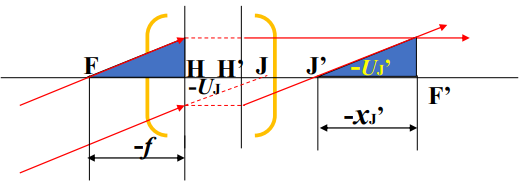
\includegraphics[width=8cm]{img/3.2.png}
            \end{figure}
由三角形全等,显然可得
\begin{align}
    x_J'={F'J'}=f \tag{3.3.1.a} \\
    X_J=FJ=f' \tag{3.3.1.b}
 \end{align}
当$f=f'$有
\begin{align}
    x_J'={F'J'}=-f'=F'H' \tag{3.3.1.a} \\
    X_J=FJ=f'=-f=FH \tag{3.3.1.b}
 \end{align}

节点$J,J'$和主点$H,H'$重合,这时光学系统两边折射率相同。


\subsubsection{理想光学系统的物像位置关系}
        \begin{figure}[H]
            \centering
            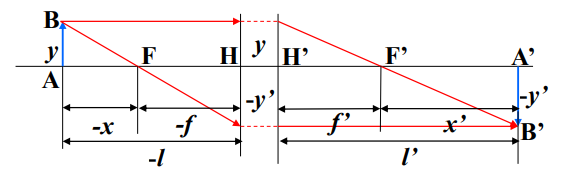
\includegraphics[width=8cm]{img/3.3.png}
            \end{figure}
最显然的我们可以得到
\begin{align}
    x x'=f f' \tag{2.3.5.a}\\
    \frac{f'}{l'}+\frac{f}{l}=1 \tag{2.3.5.b}\\
    l=x+f \quad l'=x'+f' \tag{2.3.5.c} \\
    f'n+fn'=0 \tag{2.3.5.d} \\
    \beta=\frac{nl'}{n'l}=-\frac{fl'}{f'l} \tag{2.3.5.e}
    % \frac{n'}{f'}-\frac{n}{f}=\Phi=\frac{n'}{f'}=\frac{-n}{f} \tag{2.3.5.f}
\end{align}
\begin{quote}
{\parindent2\ccwd\kaishu\zihao{5}
这里只列举一部分,就和第一章一样,参照第一章就好。
}
\end{quote}
% 将式(2.4.1.c)代入(2.4.1.a)可得(2.4.1.b)
\subsubsection{作图原则}
\begin{enumerate}[nosep]
\item 主面交点光线高度相同
\item 过节点的光线方向不变$\gamma =1$
\item 任意方向的一束平行光经理想光学系统后必交于像方焦平面上一点
\item 过物方焦平面上一点的光线经理想光学系统后必为一束平行光
\item 平行于光轴的光线经理想光学系统后必通过像方焦点
\item 过物方焦点的光线经理想光学系统后必为平行于光轴的光线
\end{enumerate}
        \begin{figure}[H]
            \centering
            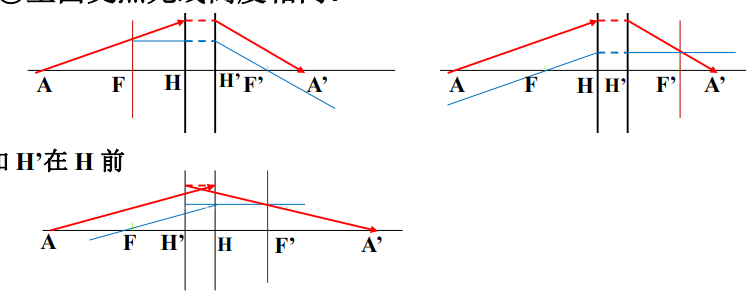
\includegraphics[width=8cm]{img/3.4.png}
            
            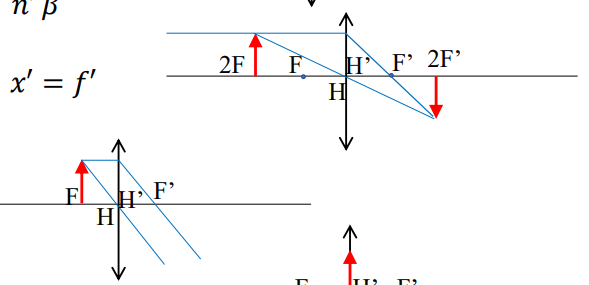
\includegraphics[width=8cm]{img/3.5.png}
        \end{figure}
\subsubsection{光束的汇聚度和系统的汇聚度}
首先直接给出几个概念
\begin{description}[nosep]% nosep没有垂直间隔
    \item[折合物距] $\displaystyle \frac{l}{n}$
    \item[折合像距]$\displaystyle \frac{l'}{n'}$
    \item[折合焦距]   $\displaystyle \frac{f'}{n'}$
    \item[汇聚度] $\displaystyle V=\frac{n}{l} \quad V'=\frac{n'}{l'}$,并且其为正代表光束是汇聚光束,反之为发散光束。
    \item[光焦度]  $\displaystyle \Phi'=\frac{n'}{f'}=\frac{-n}{f}$,正表示汇聚作用。表征光学系统偏折光线的能力。单位:屈光度——以米为单位的焦距的倒数。
\end{description}
\begin{equation}
\Phi=V'-V \tag{2.3.6}
\end{equation}
\subsubsection{透镜不同位置的成像情况}
        \begin{figure}[H]
            \centering
            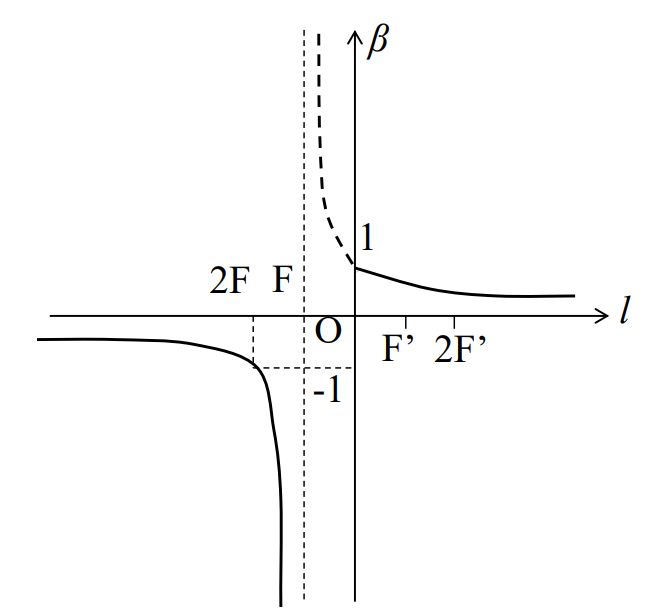
\includegraphics[width=8cm]{img/3.6.png}
            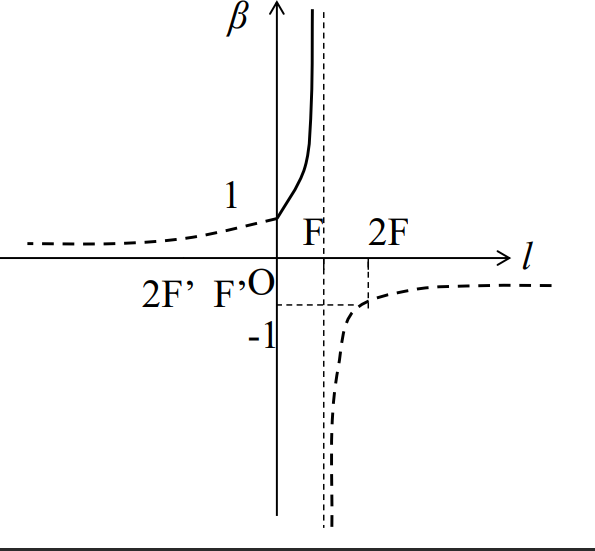
\includegraphics[width=8cm]{img/3.7.png}
            \end{figure} 
\subsection{理想光学系统的组合分析}
\subsubsection{两个理想光学系统}
图解法,任意高度做一平行于光轴的线,经过光组在像方与入射线延长线相交。得到主面,另一方同理。(根据定义,主面高度相同)
        \begin{figure}[H]
            \centering
            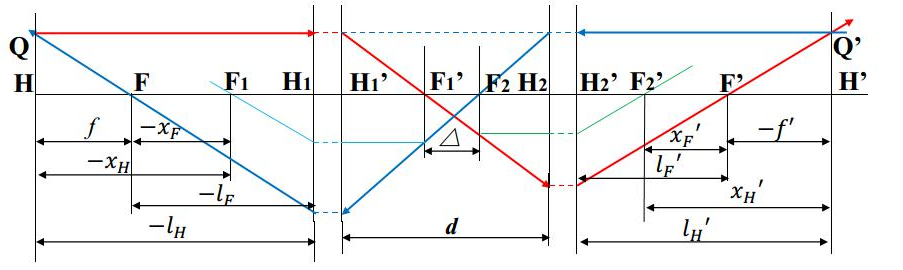
\includegraphics[width=8cm]{img/3.8.png}
            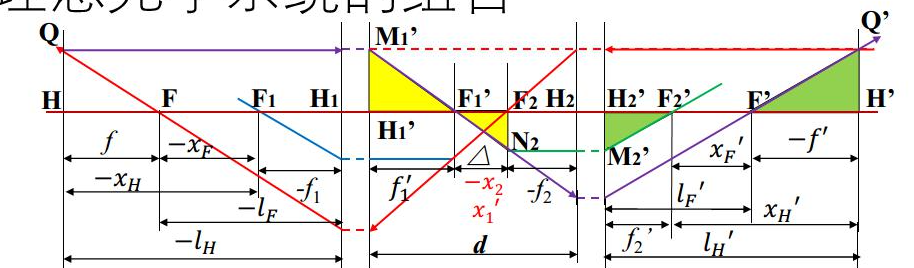
\includegraphics[width=8cm]{img/3.9.png}
        \end{figure}
然后我们对找完之后的图,来进行一下定量的分析。(以第二个光组的像方焦点、像方主点为起始点
——合成光组的物方参量 以第一个光组的物方焦点、物方主点为起始点。)直接列写
\begin{align}
    \Delta =f-f'+f_2 \tag{2.3.7.a} \\
    f=\frac{f_1f_2}{\Delta} \tag{2.3.7.b} \\
    f=\frac{-f_1'f_2'}{\Delta}\tag{2.3.7.c}
\end{align}
\subsubsection{像差和组合分析}
\section{平面与平面系统}
\section{光阑}
\begin{description}[leftmargin=1.7cm,style=nextline,nosep]% nosep没有垂直间隔
    \item[光阑 ]  光学系统中的一些中央开孔的挡光屏或光学元件的边缘。
    \item[孔径光阑    ] 限制成像光束口径的大小,
    \item[视场光阑    ] 限制成像范围的大小。
    \item[渐晕光阑
    ]遮挡轴外物体的部分光场,使像边缘模糊;

    
    \item[消杂光光阑    ]  消除镜面反射光、镜架炫光等引起的杂散光。

\end{description}
\subsection{入瞳出瞳和孔径角}
        \begin{figure}[H]
            \centering
            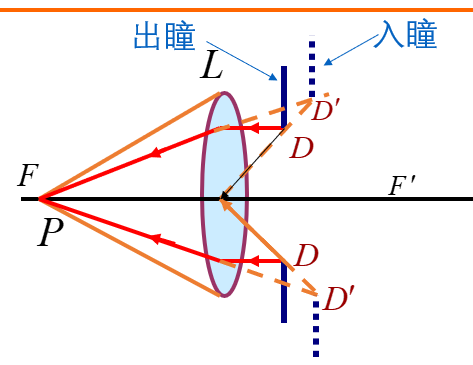
\includegraphics[width=8cm]{img/4.1.png}
            \end{figure}
入瞳是孔径光阑经过光阑后面的光学系统成的像,出瞳是经过前面的光学系统成的像。如果其在最前面,那本来就是入瞳,如果在最后面,本来就是出瞳。
\begin{description}[leftmargin=0.7cm,style=nextline,nosep]% nosep没有垂直间隔
    \item[物方孔径角] 轴上物点到入射光瞳 
\end{description}
\section{光学仪器}
\section{像差的种类和矫正}
